\documentclass[10pt,a4paper,twocolumn]{article}

\usepackage[round]{natbib}
\usepackage{crop}
\usepackage{graphicx}
\usepackage{amsmath}
\usepackage{array}
\usepackage{color}
\usepackage{amssymb}
\usepackage{flushend}
\usepackage{stfloats}
\usepackage{amsthm}
\usepackage{times}
\usepackage{tabularx}
\usepackage{pstricks}
\usepackage[left=0.75in,
 right=0.75in,
 top=1.25in,
 bottom=1.25in]{geometry}
 

\newcommand{\anote}[1]{{\color{red}[[XXX #1 ]]}} 
 
 
\begin{document}

\title{Blind dating -- A phylogenetic approach to dating HIV reservoir sequences}

\author{Joshua Horacsek$^{1,2}$, Jeffrey B. Joy$^2$, \\ Zabrina L. Brumme$^{1,2}$, and Art F.Y. Poon$^{1,2,3}$}
% 1 Simon Fraser University
% 2 BC Centre for Excellence in HIV/AIDS
% 3 University of British Columbia
\twocolumn[
  \begin{@twocolumnfalse}
    \maketitle
    \begin{abstract}
Background: The ability of HIV to persist within latent cellular reservoirs represents a major barrier to cure. The timing of establishment of individual viral reservoirs over the infection course could influence their susceptibility to elimination by immune-mediated or therapeutic approaches. However, “dating” methods to accurately estimate the age of reservoir sequences remain scarce. We propose a simple method to date suspected reservoir sequences using phylogenetic approaches. 

Method: Simulated sequence data for model validation were generated using INDELible version 1.03.  Published longitudinal clonal sequences from untreated HIV-infected individuals with estimated dates of infection were obtained from the Los Alamos National Laboratory database. Maximum-likelihood phylogenies were reconstructed with PhyML. Phylogenies were rooted by determining the location of the root that minimized the root-mean-square error between root-to-tip distances and known dates of sampling. The root-to-tip distances of latent sequences were mapped to the optimal regression line to estimate their establishment date, which was assumed to precede their sample dates by an unknown amount.
 
Results: We validated the root-to-tip method using simulated data and published longitudinal clonal sequence datasets from untreated HIV-1 infected individuals with known infection dates. For each dataset, arbitrary selections of up to 10% of sequences were handled as latent by censoring their respective sample dates.  The method accurately recovered these missing sample dates when the phylogeny conformed to a strict molecular clock, as was the case for simulated data (SOME KIND OF PERFORMANCE METRIC HERE?  MEAN RMSE?). A strict clock model could not be rejected in the majority of empirical within-host data sets. When applied to HIV DNA sequences in phylogenies containing dated HIV RNA sequences, we observed that the predicted dates tended to precede dates of sampling, which was consistent with latency (MAYBE SOME METRIC HERE LIKE MEAN DISCORDANCE).

Conclusions:
Given a known phylogeny comprised of longitudinal plasma HIV-1 RNA sequences, the establishment dates of “unknown” (reservoir) sequences can be reliably estimated when within-host HIV sequence evolution conforms to a molecular clock. Future studies will test this method on empirically derived longitudinal within-host HIV deep sequence data and extend the method to work under alternative clock models.

Keywords: 
HIV, Latency, Cellular Reservoirs, Phylogenetics, Linear Regression

    \end{abstract}
  \end{@twocolumnfalse}
]

\section{Introduction} \label{sec:intro}
Latent viral reservoirs within HIV-1 infected individuals are a major obstacle on the path to cure for HIV \citep{Pace11}. Reservoirs are cells that contain integrated viral DNA but have entered a dormant state in which they not only have a lowered rate of virion production, but can also persist within a patient for several years. Even though highly active antiretroviral therapy (HAART) can reduce a patient's viral load to below detectable levels, if a patient halts treatment latent reservoirs may reseed an infection \citep{Joos08, Pomerantz03, Richman09}.

Due to selective pressures in the host's immune system and HIV's short generation time, HIV evolves very quickly throughout the course of infection \citep{Alizon13, Shankarappa99, Rambaut04}. Once a virus has integrated itself into a cell, the rate at which it accumulates mutations becomes negligible compared to the rate at which the active population in plasma evolves. Phylogenetically, within a chronogram latency manifests as a difference between a sample's collection time and it's predicted collection time (figure \ref{fig:latenttree}). For sequences that are from the active population of virus, this assumption is reasonable.  However for sequences suspected to be latent, it is not true that the sampling time represents the time at which evolution stops.

Not much is known about the establishment of latent reservoirs over the course of an infection. The chronology of their establishment is of interest because the distribution of ages of the stored virus(es) may provide information as to the types of adaptations that the virus may have accumulated. Specifically, it may have an influence on how those infected cells react to immune-mediate or therapeutic treatments. 

Some studies have looked at the population dynamics of different classes of the virus within host, modeled them with systems of ordinary differential equations, then fit that models with empirical data \cite{Althaus14}. There has also been work that attempts to characterize latent sequences using a relaxed clock approach \cite{Immonen14}. However, there hasn't been much work towards assigning dates to sequences that are suspected to be latent, or qualitatively assessing the distribution of collection-age differences for suspected latent samples.

We propose a simple framework that utilizes the assumption of a strict molecular clock -- the expected number of substitutions per site is linearly related to time \citep{Ho14} --  on the evolution of HIV within host. Our method extracts timing information from the phylogenetic relationship between the virus sampled at various time-points along the infection. We first construct a phylogeny of plasma and PBMC samples from a patient, then calibrate a strict clock to that tree based solely on the collection dates of the plasma sequences. The root of this phylogeny is typically unknown, so we employ either root-to-tip regression or outgroup rooting to find an appropriate root. Further, we assume that PBMC cells are latent, since they contain only integrated viral DNA, and therefore have ``stopped evolving''. We do not explicitly attempt any detection of these cells. 

To assess the sensitivity of our method, we first simulated sequence data with no latent behavior and evaluated the accuracy of the reconstruction. We then simulated and evaluate sequences from a model that exhibits simplified latent behavior  \citep{Immonen14}. To mimic the types of results we expected from our first test, we used a previously published set of data to evaluate the reconstruction of dates from only plasma sequences \citep{McCloskey14}. Finally, we tested our methodology on a data-set comprised of patients that had longitudinal samples of both PBMC and plasma sequences. \anote{clean me ->} If there were pauses in evolution, provided that the molecular clock holds for all the times that the evolution has not stopped, then the clock could be a reliable source of timing for the unknown sequences. At least within the blood compartment, this should be true. 

\begin{figure} \label{fig:latenttree}
	\centering
	\scalebox{5}{%LaTeX with PSTricks extensions
%%Creator: inkscape 0.91
%%Please note this file requires PSTricks extensions
\psset{xunit=.5pt,yunit=.5pt,runit=.5pt}
\begin{pspicture}(85,53)
{
\newrgbcolor{curcolor}{0 0 0}
\pscustom[linewidth=0.38699999,linecolor=curcolor]
{
\newpath
\moveto(77.921134,4.13898)
\lineto(5.1912118,4.13898)
\lineto(5.1912118,20.207747)
}
}
{
\newrgbcolor{curcolor}{0 0 0}
\pscustom[linewidth=0.38699999,linecolor=curcolor]
{
\newpath
\moveto(65.799478,25.564002)
\lineto(29.434525,25.564002)
\lineto(29.434525,36.276514)
}
}
{
\newrgbcolor{curcolor}{0 0 0}
\pscustom[linewidth=0.38699999,linecolor=curcolor]
{
\newpath
\moveto(41.556173,46.989025)
\lineto(29.434525,46.989025)
\lineto(29.434525,36.276514)
}
}
{
\newrgbcolor{curcolor}{0 0 0}
\pscustom[linewidth=0.38699999,linecolor=curcolor]
{
\newpath
\moveto(29.434525,36.276514)
\lineto(5.1912118,36.276514)
\lineto(5.1912118,20.207747)
}
}
{
\newrgbcolor{curcolor}{0 0 0}
\pscustom[linewidth=0.38699999,linecolor=curcolor]
{
\newpath
\moveto(4.4639148,20.207747)
\lineto(5.1912118,20.207747)
}
}
{
\newrgbcolor{curcolor}{0 0 0}
\pscustom[linestyle=none,fillstyle=solid,fillcolor=curcolor]
{
\newpath
\moveto(81.87934379,5.47198716)
\lineto(81.87934379,5.02049697)
\curveto(81.73520608,5.15474288)(81.58117656,5.25507403)(81.41725524,5.32149043)
\curveto(81.25474704,5.38790683)(81.08164047,5.42111503)(80.89793554,5.42111503)
\curveto(80.53617814,5.42111503)(80.25920764,5.31018551)(80.06702402,5.08832648)
\curveto(79.8748404,4.86788057)(79.77874859,4.54851662)(79.77874859,4.13023462)
\curveto(79.77874859,3.71336575)(79.8748404,3.3940018)(80.06702402,3.17214277)
\curveto(80.25920764,2.95169685)(80.53617814,2.84147389)(80.89793554,2.84147389)
\curveto(81.08164047,2.84147389)(81.25474704,2.87468209)(81.41725524,2.94109849)
\curveto(81.58117656,3.00751489)(81.73520608,3.10784604)(81.87934379,3.24209195)
\lineto(81.87934379,2.79484111)
\curveto(81.72955362,2.69309684)(81.5705782,2.61678864)(81.40241754,2.5659165)
\curveto(81.23566999,2.51504437)(81.05903063,2.4896083)(80.87249947,2.4896083)
\curveto(80.39345355,2.4896083)(80.01615188,2.63586569)(79.74059449,2.92838046)
\curveto(79.4650371,3.22230834)(79.3272584,3.6229264)(79.3272584,4.13023462)
\curveto(79.3272584,4.63895596)(79.4650371,5.03957402)(79.74059449,5.33208879)
\curveto(80.01615188,5.62601668)(80.39345355,5.77298062)(80.87249947,5.77298062)
\curveto(81.06185686,5.77298062)(81.23990933,5.74754455)(81.40665688,5.69667242)
\curveto(81.57481755,5.6472134)(81.73237985,5.57231831)(81.87934379,5.47198716)
\closepath
}
}
{
\newrgbcolor{curcolor}{0 0 0}
\pscustom[linestyle=none,fillstyle=solid,fillcolor=curcolor]
{
\newpath
\moveto(67.94040944,25.49054575)
\lineto(67.94040944,24.41103725)
\lineto(68.57982581,24.41103725)
\curveto(68.79428027,24.41103725)(68.95281869,24.45511225)(69.05544107,24.54326224)
\curveto(69.15937912,24.63272791)(69.21134815,24.76889991)(69.21134815,24.95177825)
\curveto(69.21134815,25.13597227)(69.15937912,25.27148644)(69.05544107,25.35832076)
\curveto(68.95281869,25.44647075)(68.79428027,25.49054575)(68.57982581,25.49054575)
\lineto(67.94040944,25.49054575)
\closepath
\moveto(67.94040944,26.70227923)
\lineto(67.94040944,25.81420095)
\lineto(68.53048813,25.81420095)
\curveto(68.72520752,25.81420095)(68.86993138,25.85038191)(68.96465973,25.92274385)
\curveto(69.06070376,25.99642145)(69.10872577,26.10825353)(69.10872577,26.25824009)
\curveto(69.10872577,26.40691097)(69.06070376,26.51808522)(68.96465973,26.59176282)
\curveto(68.86993138,26.66544043)(68.72520752,26.70227923)(68.53048813,26.70227923)
\lineto(67.94040944,26.70227923)
\closepath
\moveto(67.54176097,27.02988145)
\lineto(68.56009074,27.02988145)
\curveto(68.86401086,27.02988145)(69.0982004,26.96672921)(69.26265934,26.84042474)
\curveto(69.42711828,26.71412028)(69.50934775,26.53453111)(69.50934775,26.30165725)
\curveto(69.50934775,26.12141025)(69.46724626,25.97800205)(69.38304328,25.87143266)
\curveto(69.29884031,25.76486326)(69.17516718,25.69842185)(69.01202391,25.67210842)
\curveto(69.20805897,25.63000693)(69.36001903,25.54185694)(69.4679041,25.40765844)
\curveto(69.57710484,25.27477562)(69.6317052,25.10834317)(69.6317052,24.90836109)
\curveto(69.6317052,24.64522679)(69.54223954,24.44195553)(69.36330821,24.29854734)
\curveto(69.18437688,24.15513914)(68.92979444,24.08343504)(68.59956088,24.08343504)
\lineto(67.54176097,24.08343504)
\lineto(67.54176097,27.02988145)
\closepath
}
}
{
\newrgbcolor{curcolor}{0 0 0}
\pscustom[linestyle=none,fillstyle=solid,fillcolor=curcolor]
{
\newpath
\moveto(68.8325765,47.98448198)
\lineto(68.33071752,46.62360158)
\lineto(69.33626709,46.62360158)
\lineto(68.8325765,47.98448198)
\closepath
\moveto(68.62377386,48.34897081)
\lineto(69.04321075,48.34897081)
\lineto(70.08539237,45.6143888)
\lineto(69.70075592,45.6143888)
\lineto(69.45165803,46.31589242)
\lineto(68.21898978,46.31589242)
\lineto(67.96989189,45.6143888)
\lineto(67.57976063,45.6143888)
\lineto(68.62377386,48.34897081)
\closepath
}
}
{
\newrgbcolor{curcolor}{0 0 0}
\pscustom[linewidth=0.39463133,linecolor=curcolor,linestyle=dashed,dash=0.7892628 0.7892628]
{
\newpath
\moveto(41.217255,46.97727)
\lineto(65.885506,46.9308)
}
}
\rput(42,52){\psscalebox{0.3}{$t$}}
\rput(66,52){\psscalebox{0.3}{$t^\prime$}}
\end{pspicture}
}
	\caption[Example of latent behavior]{The dotted line in the above figure is an example of latency. Sequence A was archived at time $t$, yet was collected at the same time as sequence B, at time $t^\prime$, a drift of $t^\prime - t$ is expected. If the molecular clock assumption holds true, then the date at $t$ can be inferred from }
\end{figure}

\section{Methods} \label{sec:methods}
To validate our approach, we first simulated sequence data along a phylogeny with a strict clock. We reconstructed phylogenies and randomly chose tips to censor, then reconstructed those dates from the clock. We then tested our method on patient data that was RNA only, and did the same thing, finally, we look at a homogenous dataset with both plasma and PBMC data. 

\subsection{Simulated Data} \label{subsec:simdata}
Sequences were generated in INDELible 1.03 \citep{Indelible09} along a seed phylogeny. This phylogeny was generated in TreeSim \citep{TreeSim}, and was given a clock from NESLI \citep{NELSI}. Sequences were generated using an HKY85 substitution model with parameters set from a maximum likelihood estimate from published datasets \citep{McCloskey14}. A maximum likelihood phylogeny was then reconstructed from these sequences with RAxML \citep{Raxml14}, which was then rooted using root-to-tip regression. 50 trees of 100 tips each. To test the effect of data on the clock calibration, we randomly censored the dates of 5, 10, 25 and 50 tips, then reconstructed those from the clock.

We also simulates latent behavior by randomly choosing a set number of branches, then shortening their lenghts \citep{Immonen14}.


\subsection{Data Collection} \label{subsec:dcollection}
For our second set of experiments we used a previously harvested set of data \citep{McCloskey14}. These data had been harvested from the HIV lanl database. Our third experiment also used data from Los Alamos Intra-Patient search interface \citep{LosAlamos}, except this time we used it to identify patients with both plasma and PBMC sequences from the ENV region of the HIV-1 genome. 

\subsection{Patient Data} \label{subsec:patdata}
 For our second set of experiments, we looked at RNA sequences from untreated patients from longitudinal studies with two or more clonal or single-genome (SGS) sequences available at each time point, with a known time-line relative to one of several reference points: HIV infection, seroconversion, presentation of symptomatic seroconversion illness, or birth. The seamples also were collected within 6 months (186 days) of this reference point, and where at least one of the subsequent (“follow-up”) time points occurred a minimum of 6 months after baseline. Known cases of superinfection were also excluded. 
 
We selected published studies that had well-characterized partial env sequences generated via clonal sequencing methods or single-genome amplification from HIV RNA in blood plasma or integrated DNA from PBMC cells. There was no condition for the time between sample collections. Fifteen individuals were included with serial samples from at least 3 time points (\ref{tab:patients}) \anote{This needs to be resolved, we have many samples with $2$ plasma points :/ }. A total of X partial env sequences blood plasma specimens and Y partial env sequences from PBMC cells were used in our analysis.

\begin{table*}[!ht]\label{tab:patients} 
\def\arraystretch{1.3}%
\begin{tabularx}{\textwidth}{ X | X | X | X | X | X | X } 
\hline
\hline
Patient ID & \# of plasma samples & \# of PBMC samples & Total \# of Seqeunces & \# Plasma Time points & \# PBMC time points & Total Time points   \\ \hline \hline
820$^1$ &       50 &       87 &      137 &        5 &       10 &       15  \\
821$^1$ &       76 &      192 &      268 &        7 &       17 &       17   \\ 
822$^1$ &       32 &       98 &      130 &        3 &       10 &       10   \\ 
824$^1$ &      100 &      107 &      207 &        7 &        9 &       13   \\ 
10137$^1$ &       24 &      106 &      130 &        2 &       10 &       12  \\ 
10138$^1$ &       82 &      119 &      201 &        6 &       13 &       16  \\
10586$^1$ &       16 &      121 &      137 &        2 &       12 &       14  \\ 
10769$^2$ &      229 &       96 &      325 &       10 &        4 &       11  \\ 
10770$^2$ &      190 &       31 &      221 &       11 &        2 &       11  \\ 
13889$^1$ &      151 &      132 &      283 &       13 &       14 &       18  \\ 
16616$^3$ &       16 &       95 &      111 &        2 &        5 &        5  \\ 
16617$^3$ &       16 &       89 &      105 &        2 &        5 &        5  \\ 
16618$^3$ &       25 &       75 &      100 &        2 &        5 &        6  \\ 
16619$^3$ &       13 &       60 &       73 &        2 &        6 &        6  \\ 
34382$^4$ &       37 &        5 &       42 &        3 &        1 &        4  \\ 
34391$^4$ &       13 &       38 &       51 &        3 &        5 &        6  \\ 
34393$^4$ &       25 &       74 &       99 &        2 &        6 &        7  \\ 
34396$^4$ &       23 &       46 &       69 &        2 &        5 &        5 \\ 
34397$^4$ &       26 &       25 &       51 &        2 &        2 &        4  \\ 
34399$^4$ &       61 &       88 &      149 &        5 &        9 &       12  \\ 
34400$^4$ &       54 &       23 &       77 &        4 &        1 &        5  \\ 
34405$^4$ &       27 &       29 &       56 &        3 &        2 &        4  \\ 
34408$^4$ &        5 &       73 &       78 &        2 &        8 &        8 \\ 
34410$^4$ &       35 &       60 &       95 &        2 &        6 &        6 \\ 
34411$^4$ &       25 &       43 &       68 &        3 &        3 &        6   \\ \hline \hline
\end{tabularx}

  \caption{$^1$ \cite{Shankarappa99}, $^2$ \cite{Fischer04}, $^3$ \cite{Llewellyn06},  $^4$ \cite{Novitsky09} --  patient data collected from the HIV LANL database \citep{LosAlamos}}
\end{table*}

\subsection{Sequence Aligment} \label{subsec:seqalign}
All of our sequences were annotated in FASTA formats, each containing multiple time points. Our simulated sequences were not simulated with any insertions or deletions, and no alignment was necessary, additionally, the dataset we used for our second set of experiments was already cleaned and aligned \citep{McCloskey14}. For our third dataset, we used the built in MUSCLE \citep{Muscle04} interface within AliView \citep{AliView14} to align the sequences, which were then visually inspected and modified. 

\subsection{Phylogenetic Reconstruction} \label{subsec:phylo}
In all experiments all of our reconstructed phylogenies were maximum likelihood phylogenies reconstructed in RAxML \citep{Raxml14} using the GTR+$\Gamma$ model. Synthetic data were solely rooted with root-to-tip regression. For all other patient data, both outgroup rooting (against the HIV-1 B ancestor consensus \citep{HIVBANC} \anote{what's the correct reference here}) and root-to-tip regression \cite{Ape04} were used to root the tree. We did not attempt to use BEAST \citep{BEAST} to build any phylogenies, as leaving dates unspecified on the amount of tips we had drastically increases the dimensionality of the problem, and would need a prohibitively large amount of samples from the MCMC chain to converge.

\subsection{Date Reconstruction} \label{subsec:daterecon}
Once the trees had been rooted, a general linear model with the normal family was constructed with the with expected number of substitutions as the input, and sampling time as the response. For all experiments using patient data, this fit was only over the plasma data, and the PBMCs expected subs were used as input. From this, we collected the difference between the observed sampling date, and the predicted date. 


\subsection{Patient Rejection} \label{subsec:hypot}
\anote{Patients whose linear model. Log ratio test. alpha value of 0.01\%.}

\section{Results} \label{sec:results}
Our first validation experiment on synthetic data was preformed as such: First we choose 50\% of the tips of a phylogeny and censored those dates, we next used root-to-tip regression \citep{APE} on the remaining data to calibrate the molecular clock for the tree. Finally, for each censored date, we reconstructed the expected date using the expected number of substitutions.

In all of our experiments, before any analysis is done, all times are re-scaled to lie between $0$ and $1$. This is calculated as $$ \text{new time} = \frac{\text{time} - \text{min time}}{\text{max time} - \text{min time}}$$ this gives normalized time. Errors are then calculated from this number, which we call normalized error. On the left figure \ref{fig:results1} shows a linear regression over either simulation time or time from a reference point (for patient data). On the right side of figure \ref{fig:results1}, is the superposition of an error density estimate for each data set within a category. 

\begin{figure*}[!ht] \label{fig:results1}
	\centering
	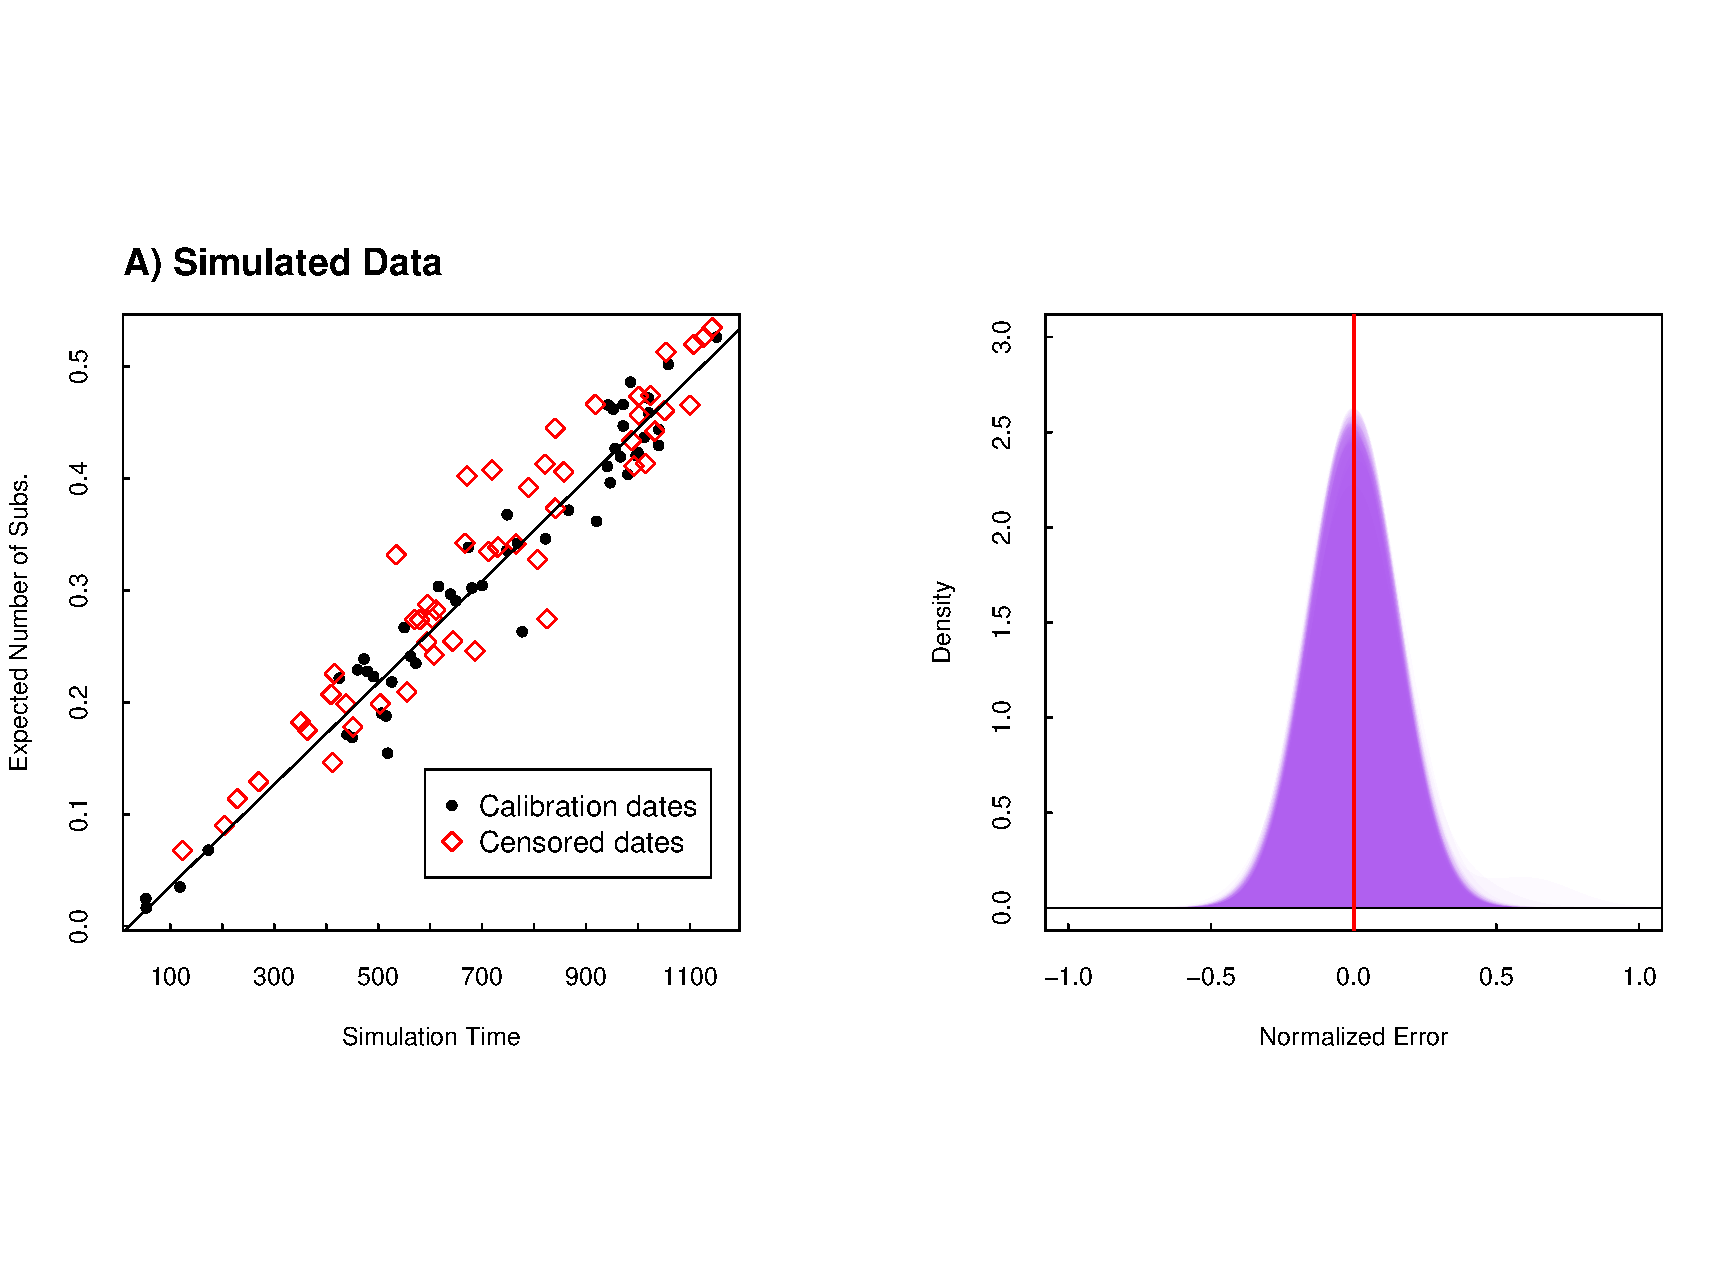
\includegraphics[trim=0cm 0cm 0cm 6cm, clip=true, scale=0.425]{figures/simulated.pdf} \\
	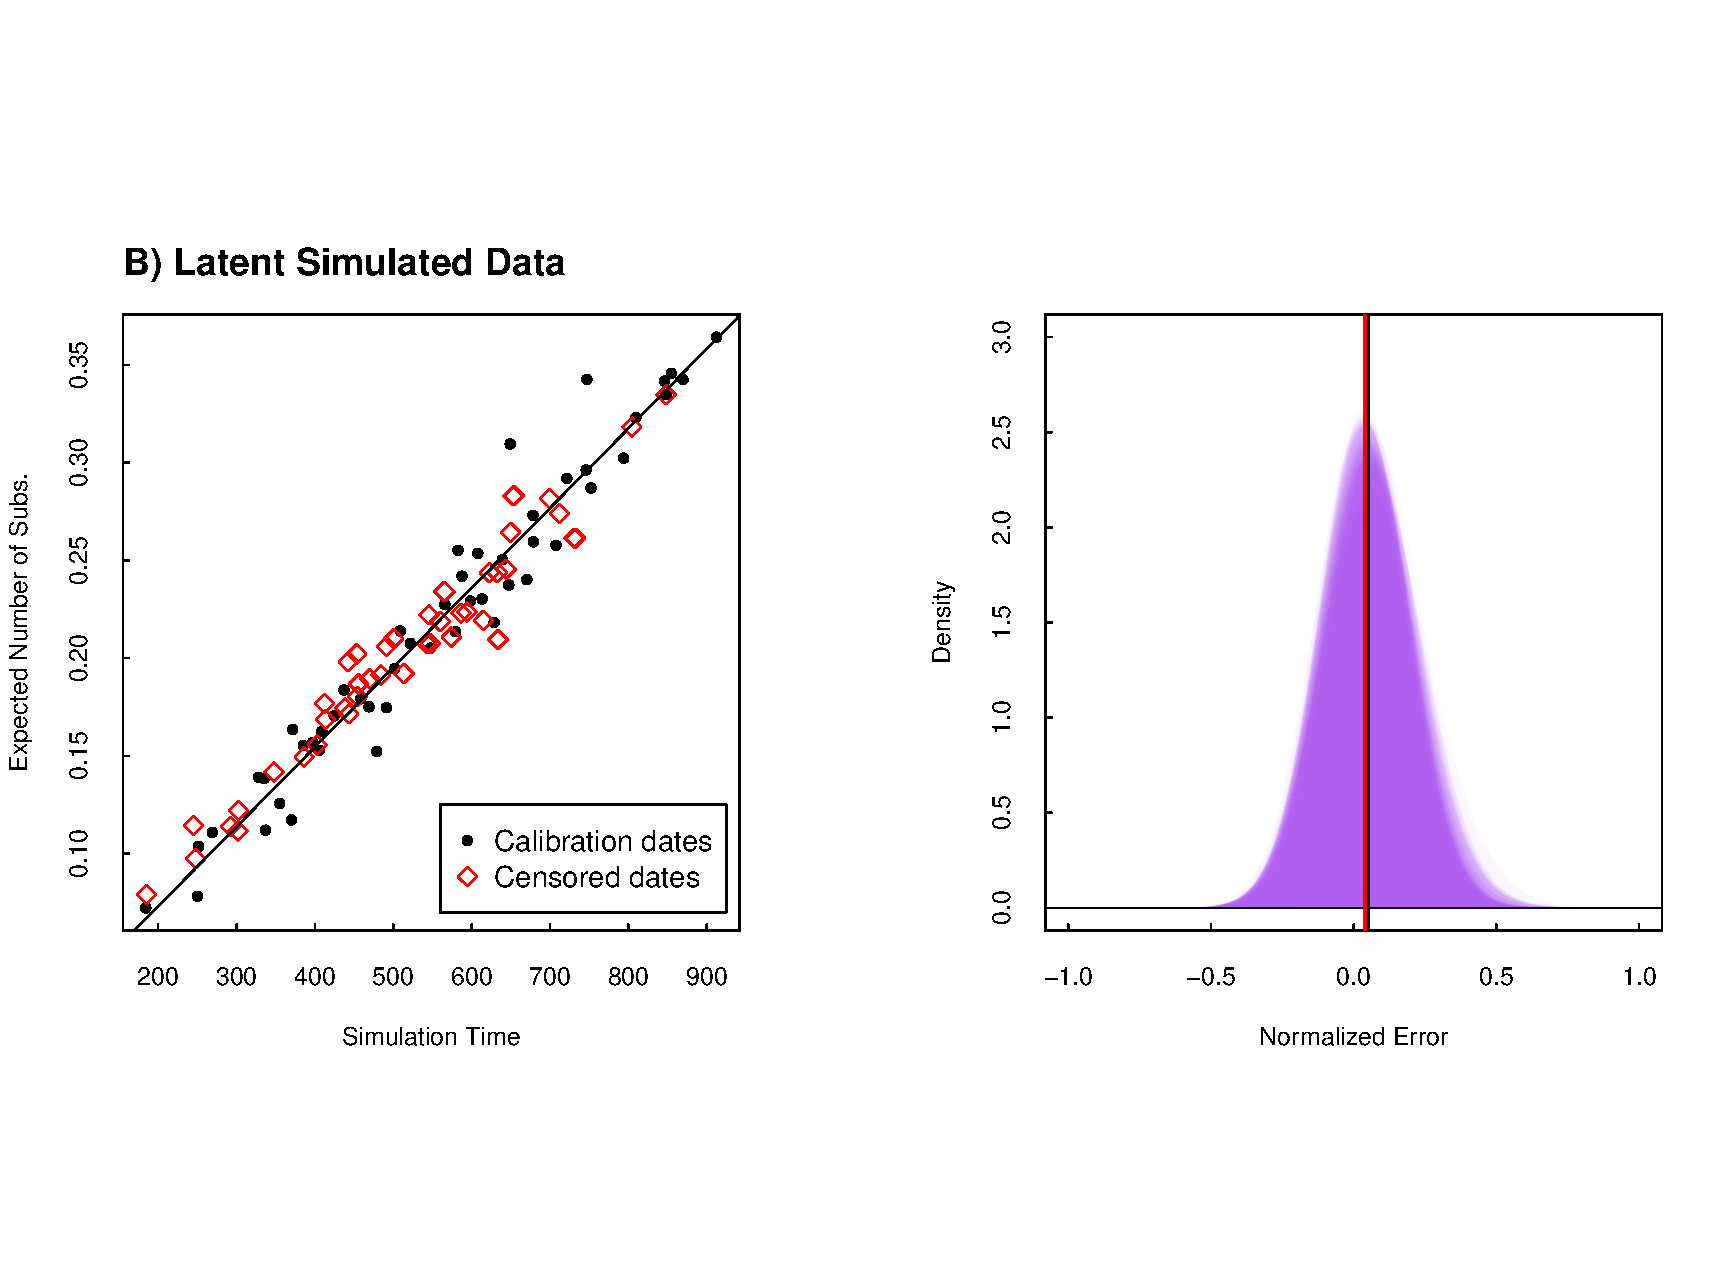
\includegraphics[trim=0cm 0cm 0cm 7cm, clip=true,scale=0.425]{figures/simulated_latent.pdf}\\
	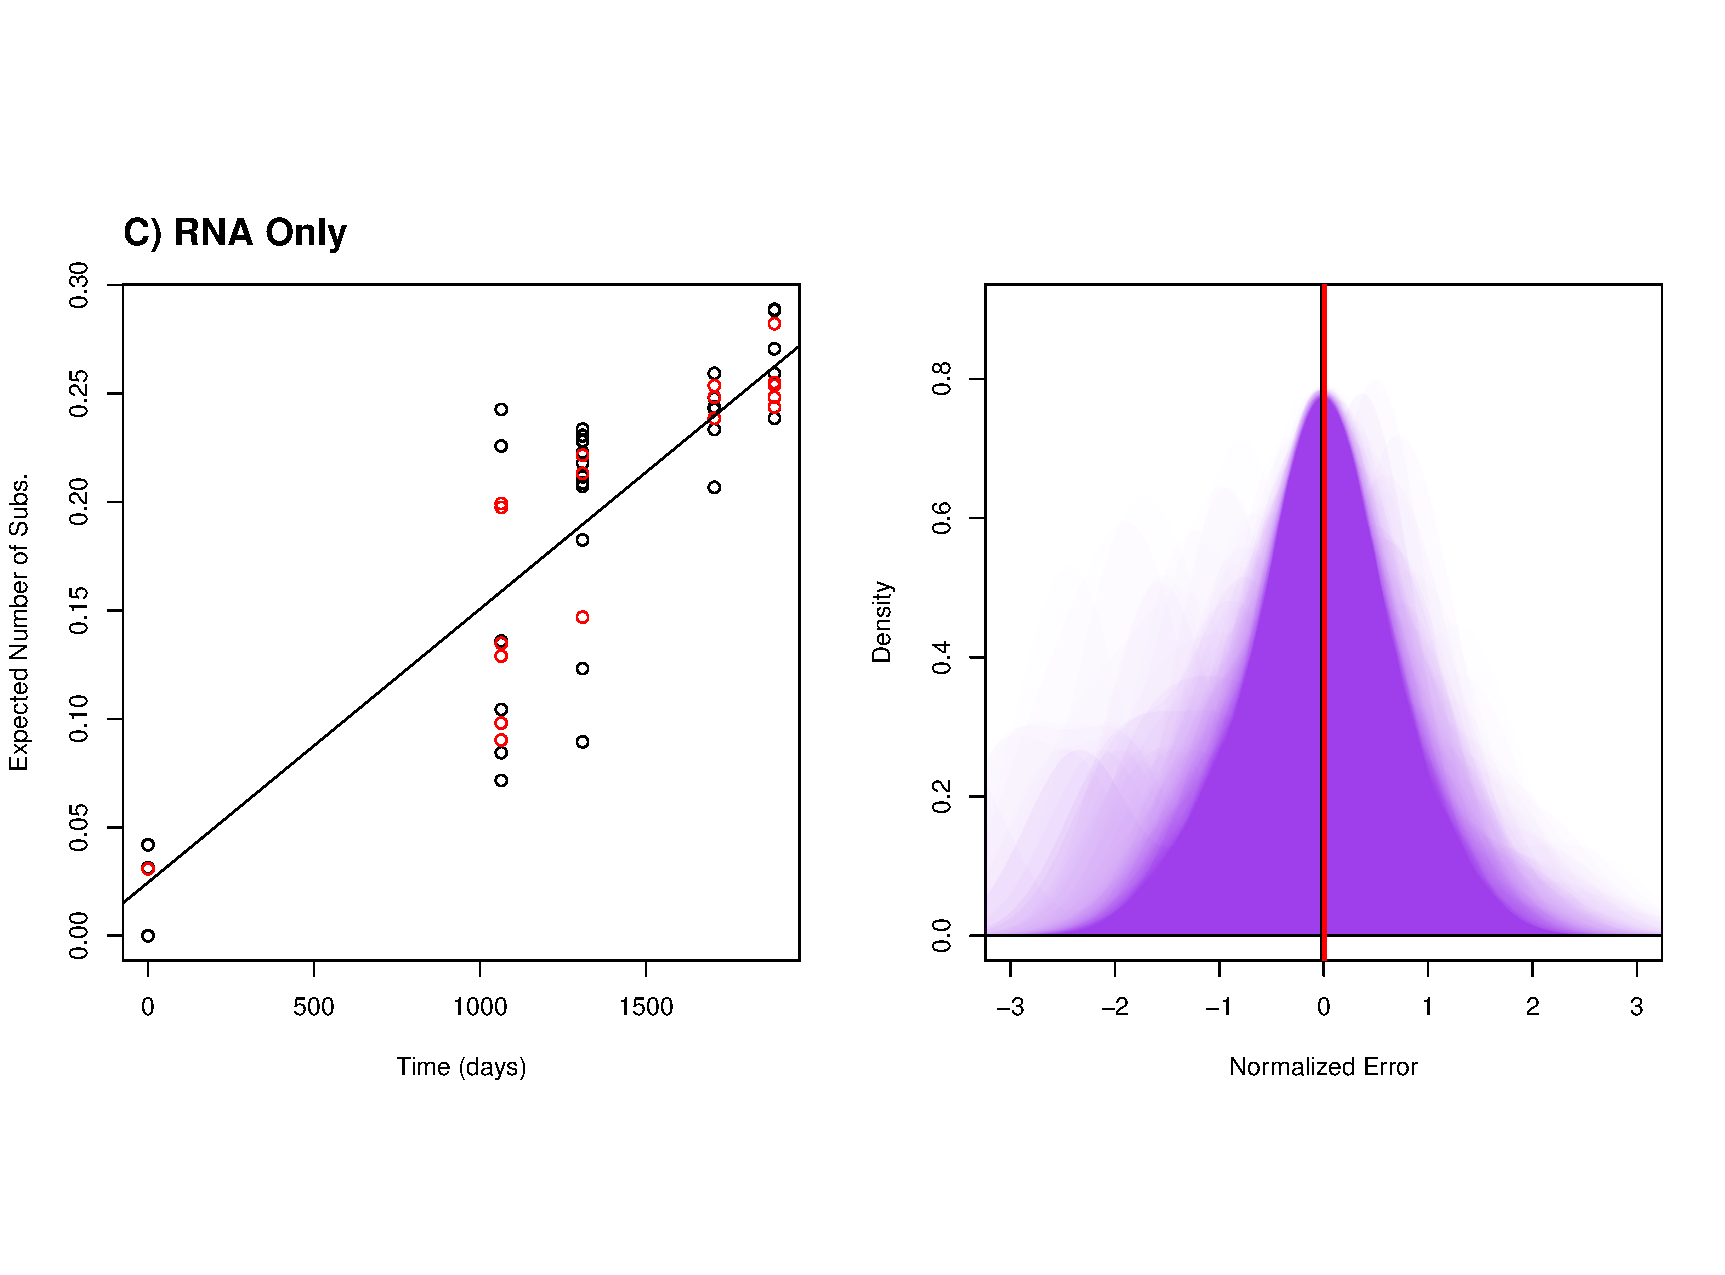
\includegraphics[trim=0cm 0cm 0cm 7cm, clip=true,scale=0.425]{figures/ancre.pdf}\\
	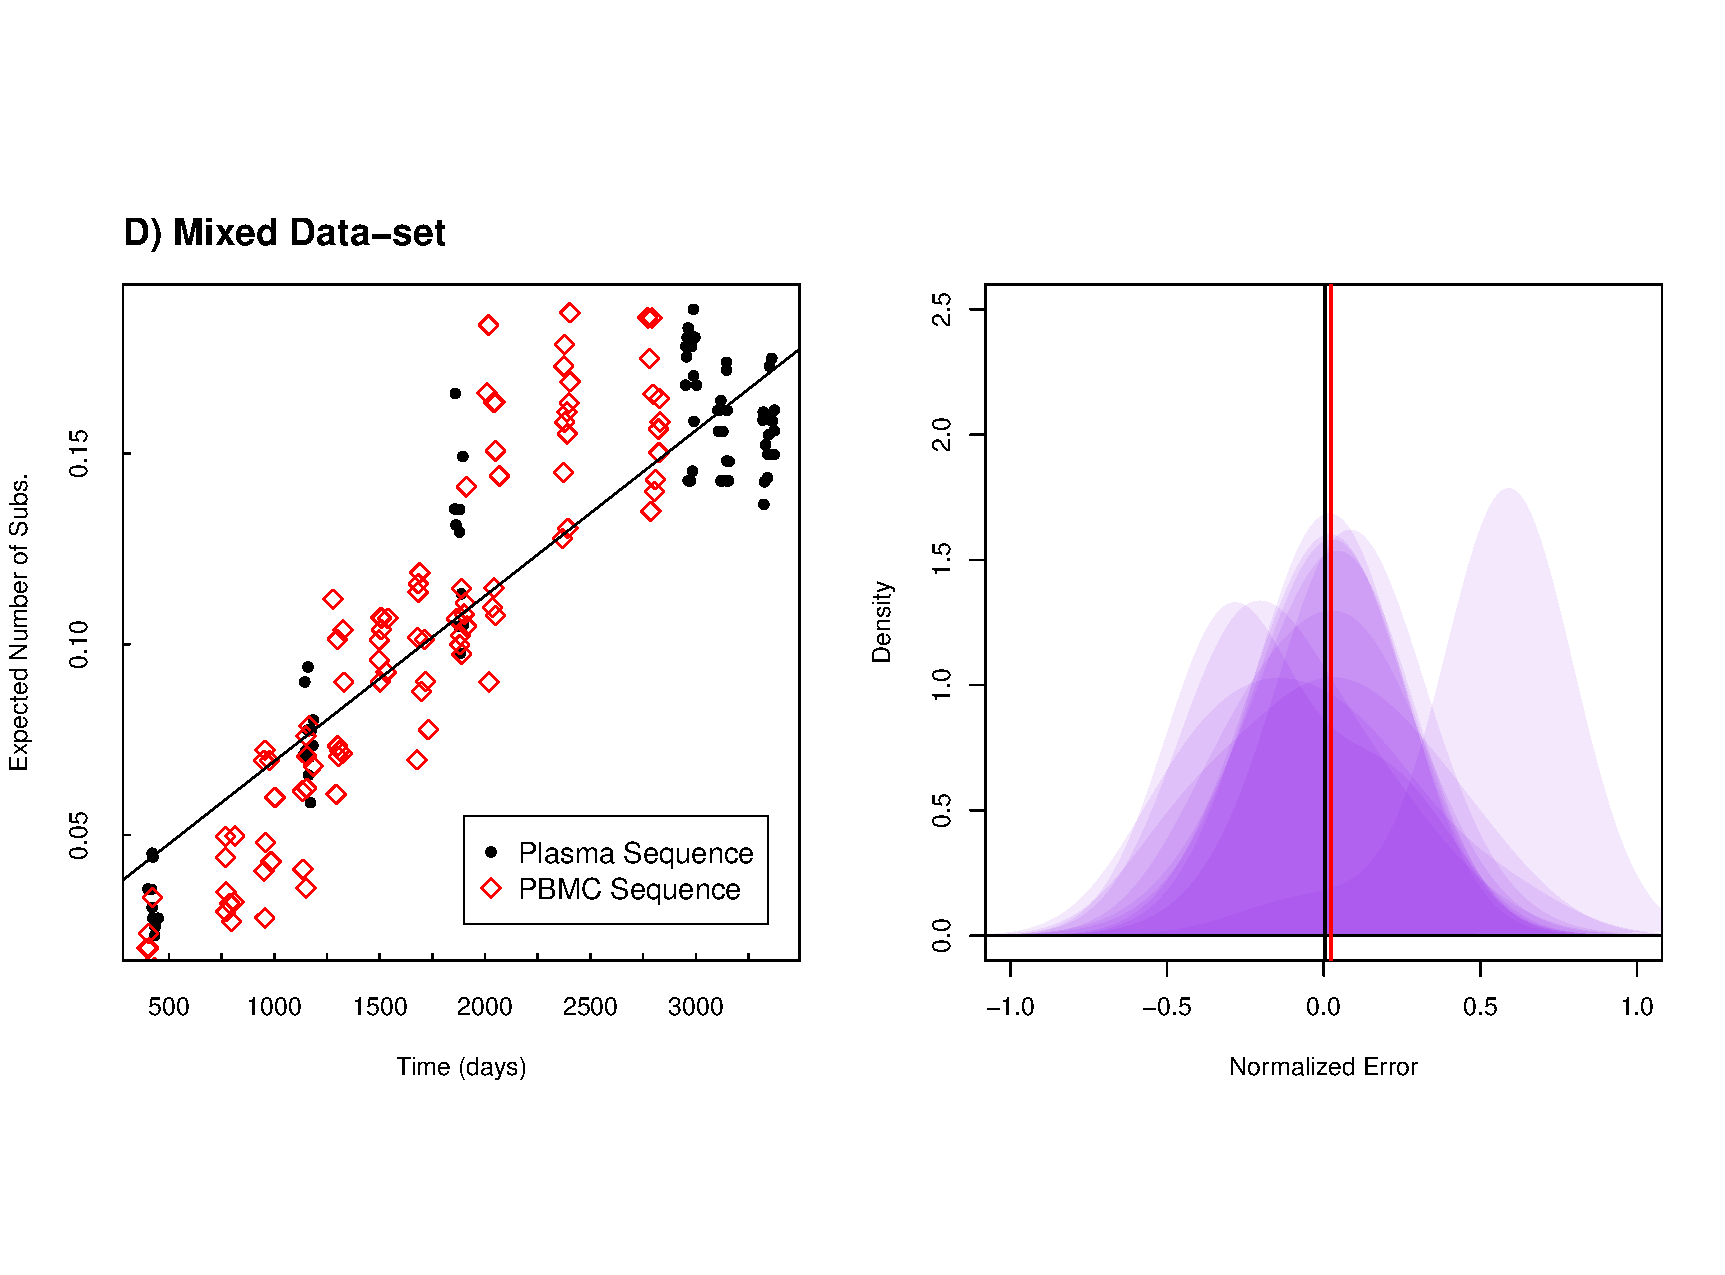
\includegraphics[trim=0cm 4cm 0cm 7cm, clip=true,scale=0.425]{figures/lanl.pdf}
	\caption[Examples]{\anote{Add legend, change points, change shading, explain point colouring, explain mean and median lines.}}
\end{figure*}


\subsection{Simulated Data} \label{sec:sim_results}
For our simulated data, we evaluated three error metrics. We looked at the mean square error for each synthetic tree, as well as the mean and median difference between the predicted date and sampling date. Figure \ref{fig:results1} A) shows that the clock is a reliable source of information in this case. Quantitatively, the censored data points are close to the regression line, and the difference density is heavily peaked around 0. Averaged over all simulated data sets, the average mean square error was \anote{X}, and the average median and mean difference were \anote{Y} and \anote{Z} respectively.

We evaluated the latent simulated data under similar metrics. Figure \ref{fig:results1} B) shows the regression over the calibration dates and the simulated collection dates. Note that these dates are not the actual. In this experiment, the density plot is shifted to the right, exemplifying latent behavior. Averaged over all simulated data sets, the average mean square error was \anote{X}, and the average median and mean difference were \anote{Y} and \anote{Z} respectively. However, when we utilized the known sample ages (as opposed to the collection dates) then measured the same metrics, averaged over all simulated data sets, the average mean square error was \anote{X}, and the average median and mean difference were \anote{Y} and \anote{Z} respectively.

\subsection{RNA Only Data} \label{sec:rna_only}
To evaluate the possible effectiveness of this methodology on real data, we utilized the plasma only data set \citep{McCloskey14}. For every applicable patient, we censored 50\% of their known sampling dates then reconstructed the censored dates using the linear model calibrated over the uncensored dates. We also performed this experiment with RTT rooting and out group rooting \anote{we should have another figure like figure 2 for both RTT and out-group rooting}. The goal of this experiment was to parallel the type of results from \ref{sec:sim_results}.

Figure \ref{fig:results1} C) shows the regression over the calibration dates and the collection date. Averaged over all simulated data sets, the average mean square error was \anote{X}, and the average median and mean difference were \anote{Y} and \anote{Z} respectively. The superposition of the difference density plots shows similar behavior to that of \ref{sec:sim_results}, except with a wider distribution, and more variation. Since there is inherently more noise in this data, this is expected. 

\subsection{Patient Reconstruction}
Finally, we looked at patients who had both plasma and PBMC samples available. We used both RTT and outgroup rooting to root the phylogeny, then calibrated a clock to the known plasma sampling dates and reconstructed the expected age of the sequences for all patients who could reject the null model \ref{subsec:hypot}. 

Figure \ref{fig:results1} D) shows the regression over the calibration dates and the simulated collection date. In this case, we do not know the actual date of archival.  The superposition of the difference density plots shows similar behavior to that of the latent simulated data, except \anote{need new plots for this}.

The patients that had received treatment at some point generally failed the hypothesis testing -- there was only one patient that did not. This suggests that after a patient begins treatment, the assumption of a molecular clock over their phylogeny is too strong. 

\section{Discussion} \label{sec:discuss}
The simulated data are unsurprising, the RNA data too. Patient data trends and analysis.
\section{Conclusion} \label{sec:conclusion}
In this work we showed that a phylogeny's clock, when reliable, is a valuable source of information with respect to dating sequences that are suspected to show latent behaviour in patients infected with HIV-1. 
Via simulation, we built phylogenies that adhered to clock-like behaviour, with and without latent sequences.
From those, were able to reliably reconstruct dates for both active and latent sequences, rooting the trees via root-to-tip regression.
Then, using real data, we performed analogous reconstructions, using both root-to-tip regression and outgroup rooting, and showed similar results.

However, there are ways in which this method could be improved. 
These results hinge on the strong assumption of a molecular clock over the data, which is not always true. 
It may be possible to adapt a maximum likelihood relaxed clock methodology with this approach, giving more flexibility over noisy or unreliable data. 
Additionally, we would like to apply the methodology to next gen sequence data -- we would like to see if mass amounts of short read data contain sufficient information to calibrate the clock.


\section{Acknowledgments} \label{sec:ackn}
The authors would like to thank --.

\bibliographystyle{natbib}
%\bibliographystyle{achemnat}
%\bibliographystyle{plainnat}
%\bibliographystyle{abbrv}
%\bibliographystyle{bioinformatics}
%\bibliographystyle{plain}

\bibliography{main}

\end{document}
